\section{Optymalizacja układu geometrycznego}
\label{sec:construction_optymization}
\begin{figure}[htbp]
\centering
\fbox{BADANE UKŁADY GEOMETRYCZNE - szkic }%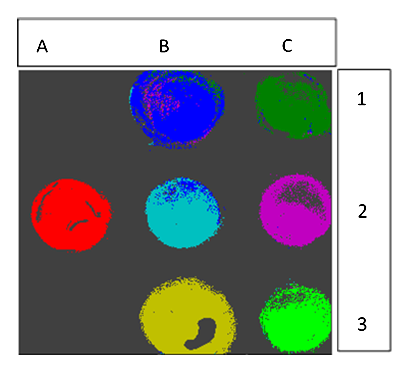
\includegraphics[width=\linewidth]{sample}}
\caption{Szkic badanych układów konstrukcyjnych sensorów piezoelektrycznych.}
\label{fig:construct_scetch}
\end{figure}
Niełatwe rozważania na temat kierunku badań dotyczących konstrukcji sensora zaowocowały ustaleniami o konieczności zbadania przetwornika:
\begin{enumerate}
\item belkowego ze względu na możliwość odniesienia się do istniejącej literatury(patrz: A na Rys.\ref{fig:construct_scetch}),
\item o kształcie rury z powodu przeznaczenia konstruowanego przetwornika (patrz: B na Rys.\ref{fig:construct_scetch}),
\end{enumerate}